\subsection{Day 1} \label{sec:day1}

The daily meeting took place as planned at 11:00 PST.\footnote{\url{https://confluence.lsstcorp.org/display/DM/OPS+Rehearsal+\%28Day+1\%3A+2020-07-28\%29+Meeting+notes}}

Bias, Flat, and Dark sequences were acquired.  A clear problem, L3 fogging, was
noted and resulted in the replacement of the N2 bottle.  It was noted that
fogging was clearing and flats on subsequent nights should show a change
(which did indeed turn out to be the case, \figref{fig:d1}).

Transfers showed problems with roughly 25s per file (CCD).  The $\sim$30 exposure
required O(1.5 hours) to reach the USDF.  On arrival problems were detected with
the ingestion of data.  The culprit was that two processes were trying to ingest
incoming files (one linking them with a deprecated file path).  Once transfers
completed, data repositories were regenerated fixing the issue.

Processing proceeded rapidly.  Jobs were submitted using parallelism over 9 CCDs
making up the ComCam raft.  Total processing time was O(15 minutes) using 10 cores.
There were problems with calibration ingestion (the CALIB area does not have
permissions to allow group access).  It is suspected that this has caused preliminary
calibration based on early ComCam tests from a few weeks prior to be used in the
reduction of the new calibration data but current provenance did not show
which calibrations were used.

QA was performed with notebooks  and shared.  This analysis demonstrated that the
proper calibrations were not used , as evidenced by bias-like patterns printing through on the “calibrated” dark frames (\figref{fig:d2}).

\begin{figure}
\begin{center}
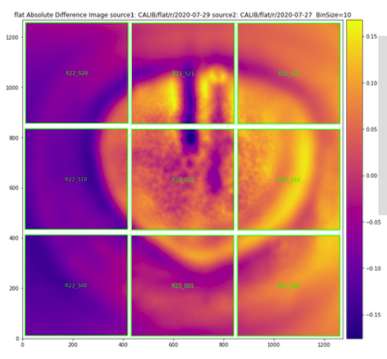
\includegraphics[width=0.9\textwidth]{figures/n1moist}
\end{center}
\caption{Left: Night 1 flat with moisture on L3 lens.  Right: Night 2 flat with moisture now cleared.\label{fig:d1}}
\end{figure}

\subsubsection{Discussion}
We discussed how to implement needed changes in infrastructure to support the current
Butler Gen2 usage of calibrations (group write permissions were extended for the
interim).  Further discussions about Gen2 vs. Gen3 and the level of sophistication
to plan for the next rehearsal.

